\documentclass[a4paper]{article}
\usepackage[spanish, es-lcroman]{babel}   % es-lcroman: for roman in lower-case in enumerate
\usepackage{graphicx}
\pagestyle{headings}
\titlepage
\usepackage[utf8]{inputenc} 		% para codificacion unicode (utf8)
\usepackage{enumerate}
\usepackage{hyperref}			% para links a paginas web
\usepackage{subfig}
\usepackage{graphics}
\usepackage{amsmath}
\usepackage{amssymb}
\usepackage{amsthm}
%\usepackage{placeins}
\usepackage{tabularx}
\usepackage{booktabs,siunitx}
%\usepackage{fullpage}

\decimalpoint

% That follow if for listings configuration
\usepackage{listings}
\usepackage{color}
\usepackage{textcomp}
\definecolor{listinggray}{gray}{0.9}
\definecolor{lbcolor}{rgb}{0.99,0.99,0.99}
\lstset{
    backgroundcolor=\color{lbcolor},
    tabsize=4,
    rulecolor=,
    language=matlab,
        basicstyle=\scriptsize,
        upquote=true,
        aboveskip={1.5\baselineskip},
        columns=fixed,
        showstringspaces=false,
        extendedchars=true,
        breaklines=true,
        prebreak = \raisebox{0ex}[0ex][0ex]{\ensuremath{\hookleftarrow}},
        frame=single,
        showtabs=false,
        showspaces=false,
        showstringspaces=false,
        identifierstyle=\ttfamily,
        keywordstyle=\color[rgb]{0,0,1},
        commentstyle=\color[rgb]{0.133,0.545,0.133},
        stringstyle=\color[rgb]{0.627,0.126,0.941},
}

\newcommand{\X}{\mathbf{X}}
\newcommand{\V}{\mathbf{V}}
\newcommand{\W}{\mathbf{W}}
\newcommand{\Hbf}{\mathbf{H}}
\newcommand{\vbf}{\mathbf{v}}
\newcommand{\h}{\mathbf{h}}
\newcommand{\A}{\mathbf{A}}
\newcommand{\B}{\mathbf{B}}
\newcommand{\x}{\mathbf{x}}

\DeclareMathOperator*{\argmin}{arg\,min}
\DeclareMathOperator*{\argmax}{arg\,max}

\newtheorem*{theorem*}{Teorema}

\title{Filtro acoplado}
\author{Ernesto López}

\begin{document} 

\maketitle

\section{Introducción}

En un sistema de comunicación digital, el receptor óptimo es aquel que produce mínima probabilidad de error de detección de bits. Si el sistema es en banda base, el receptor óptimo es el \textbf{filtro acoplado}, también llamado filtro adaptado (\emph{matched filter} en inglés). En este documento se presenta la teoría sobre el filtro acoplado. Se deduce también la probabilidad de error en un sistema de comunicación de transmisión digital en banda base \(M\)-ario.

Lo incluido en este documento constituye una parte de un tema de un curso sobre sistemas de comunicación. Todo lo aquí presentado está basado en los capítulos 9 y 11 del libro \cite{Carlson2009}.

\section{Detección de pulsos y filtro acoplado}

En un sistema de comunicación binario, la información se transmite como un \textbf{0} o un \textbf{1} durante un intervalo de tiempo \(T_b\). Típicamente, cada bit se codifica como un pulso analógico de forma de onda \(p(t)\) fija con soporte de duración \(T_b\) o menor, multiplicado por una constante que depende del bit transmitido. Por ejemplo, en un sistema binario con codificación de línea polar, la amplitud del pulso se multiplica por \(A/2\) para transmitir un 1 y por  \(-A/2\) para transmitir un 0. El receptor recibe los pulsos contaminados con ruido y debe detectar la presencia de cada uno así como su amplitud para determinar cuales fueron los bits transmitidos. Para esto, el filtro en el receptor se diseña de forma de resaltar el pulso y atenuar el ruido lo mas posible. Muestreando la señal filtrada en instantes adecuados y evaluando la amplitud de la muestra, se determina cual fue el bit transmitido. Cuando se conoce la forma del pulso, es posible diseñar filtros de recepción óptimos para detectar pulsos contaminados con ruido aditivo de cualquier densidad espectral de potencia  (PSD, \emph{Power Spectral Density}) conocida. A continuación se desarrolla el diseño del filtro receptor óptimo.

Como primera aproximación al problema, se considera el caso en que se quiere diseñar el filtro en el receptor con el único objetivo de detectar la llegada de un pulso contaminado con ruido aditivo. El pulso recibido tiene forma \(p(t)\) conocida, pero amplitud \(A_p\) y tiempo de llegada \(t_0\) desconocidos. Por lo tanto, la señal recibida es
\begin{equation}\label{eq:xr}
 x_R(t)=A_pp(t-t_0).
\end{equation}
Para detectar el pulso, el filtro del receptor debe maximizar la amplitud pico de la salida producida por el pulso y a su vez minimizar la potencia del ruido. Es decir, el filtro del receptor tiene que maximizar la \textbf{relación amplitud pico de señal a potencia de ruido}. Se quiere encontrar la función de transferencia \(H(f)\) del filtro del receptor que logre este objetivo conociendo la forma del pulso \(p(t)\) y la PSD \(G_{n_R}(f)\) del ruido. En la figura \ref{fig:matched_filter_scheme} se ilustra la situación en el caso en que el pulso \(p(t)\) es rectangular.
\begin{figure}[!htb]
\begin{center}
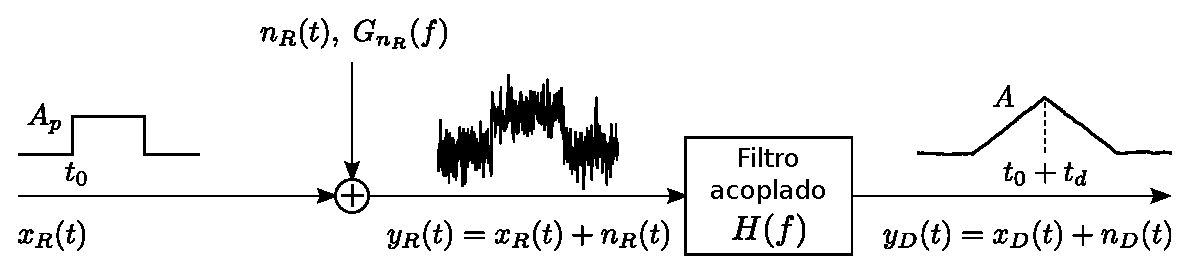
\includegraphics[width=0.9\columnwidth]{figuras/matched_filter_scheme_v2.eps}
\caption{\label{fig:matched_filter_scheme} Esquema del filtro acoplado. El filtro debe maximizar la relación amplitud pico de la señal a potencia de ruido. Dada la llegada de un pulso en el tiempo \(t_0\), el filtro se diseña para maximizar la amplitud \(A\) del pulso filtrado en cierto instante \(t_d\) luego de la llegada del pulso, teniendo en cuenta que a la vez debe minimizar la potencia del ruido.}
\end{center}
\end{figure}

El análisis se realizará en el dominio de la frecuencia. Si la transformada de Fourier de \(p(t)\) es \(P(f)\), empleando la propiedad de desplazamiento temporal de la transformada de Fourier, se deduce que la transformada de Fourier de la señal recibida \(x_R(t)\) es
\begin{equation}\label{eq:xr_frequency}
 X_R(f)=A_pP(f)e^{-j2\pi ft_0}.
\end{equation}
Sea \(x_D(t)\) la salida del filtro producida por la señal recibida \(x_R(t)\). En el dominio de la frecuencia, se cumple que
\[
 X_D(f)=H(f)X_R(f).
\]
Se quiere maximizar la amplitud pico \(A\) de \(x_D(t)\) en cierto instante específico, por ejemplo, en \(t=t_0+t_d\), como se muestra en la figura \ref{fig:matched_filter_scheme}. Operando, se tiene que
\begin{align*}
 A &= x_D(t_0+t_d)\\
    &=\mathcal{F}^{-1}\left[X_D(f)\right]\Big|_{t=t_0+t_d}\\
    &=\mathcal{F}^{-1}\left[H(f)X_R(f)\right]\Big|_{t=t_0+t_d}\\
    &=\left[\int_{-\infty}^{\infty}H(f)X_R(f)e^{j2\pi ft}\,df\right]\bigg|_{t=t_0+t_d}\\
    &=\int_{-\infty}^{\infty}H(f)X_R(f)e^{j2\pi f(t_0+t_d)}\,df,
\end{align*}
y usando la ecuación \ref{eq:xr_frequency} se concluye que la amplitud pico se puede expresar como
\begin{equation}\label{eq:peak_amplitude_detected}
 A=A_p\int_{-\infty}^{\infty}H(f)P(f)e^{j2\pi ft_d}\,df.
\end{equation}
Por otro lado, teniendo en cuenta que la PSD del ruido filtrado es
\[
 G_{n_D}(f)=\left|H(f)\right|^2G_{n_R}(f),
\]
la potencia del ruido filtrado es\footnote{Se asume que el ruido contaminante es de media nula y por lo tanto, el ruido filtrado también es media nula, así que la potencia coincide con la varianza.}
\begin{equation}\label{eq:noise_power_detected}
 P_{n_D}=\sigma^2=\int_{-\infty}^{\infty}\left|H(f)\right|^2G_{n_R}(f)\,df.
\end{equation}
Se quiere encontrar \(H(f)\) de forma de maximizar la relación amplitud pico de señal a potencia de ruido \((A/\sigma)^2\), que usando las ecuaciones \ref{eq:peak_amplitude_detected} y \ref{eq:noise_power_detected} es 
\begin{equation}\label{eq:signal_peak_noise_relation_generic}
 \left(\frac{A}{\sigma}\right)^2=\frac{A_p^2\left|\displaystyle\int_{-\infty}^{\infty}H(f)P(f)e^{j2\pi ft_d}\,df\right|^2}{\displaystyle\int_{-\infty}^{\infty}\left|H(f)\right|^2G_{n_R}(f)\,df}.
\end{equation}
El problema puede resolverse de forma directa usando la desigualdad de Schwarz. La desigualdad de Schwarz indica que para cualquier par de funciones \(V(f)\) y \(W(f)\) complejas y cuadrado integrables, se cumple que
\[
\left|\int_{-\infty}^{\infty}V(f)W^*(f)\,df\right|^2\leq \int_{-\infty}^{\infty}\left|V(f)\right|^2\,df \int_{-\infty}^{\infty}\left|W(f)\right|^2\,df,
\]
y se verifica la igualdad si \(V(f)\) es proporcional a \(W(f)\), es decir, si \(V(f)=K'W(f)\), con \(K'\) una constante. Planteando la desigualdad como
\begin{equation}\label{eq:schwarz_inequality}
\frac{\left|\displaystyle\int_{-\infty}^{\infty}V(f)W^*(f)\,df\right|^2}{\displaystyle\int_{-\infty}^{\infty}\left|V(f)\right|^2\,df}\leq \int_{-\infty}^{\infty}\left|W(f)\right|^2\,df, 
\end{equation}
y tomando
\begin{align*}
 V(f)&=H(f)\sqrt{G_{n_R}(f)}\\
 W^*(f)&=\frac{A_pP(f)e^{j2\pi ft_d}}{\sqrt{G_{n_R}(f)}},
\end{align*}
el lado izquierdo en la desigualdad de la ecuación \ref{eq:schwarz_inequality} coincide con \((A/\sigma)^2\) (ecuación \ref{eq:signal_peak_noise_relation_generic}). Por lo tanto, la desigualdad de Schwarz permite acotar  a \((A/\sigma)^2\) como
\begin{equation*}
 \left(\frac{A}{\sigma}\right)^2 \leq A_p^2\int_{-\infty}^{\infty}\frac{\left|P(f)\right|^2}{G_{n_R}(f)}\,df.
\end{equation*}
La igualdad en esta ecuación es la máxima relación amplitud pico a potencia de ruido que se puede alcanzar,
\begin{equation}\label{eq:signal_peak_noise_relation_optimal}
 \left(\frac{A}{\sigma}\right)_\textrm{máx}^2 = A_p^2\int_{-\infty}^{\infty}\frac{\left|P(f)\right|^2}{G_{n_R}(f)}\,df.
\end{equation}
y se da cuando \(V(f)=K'W(f)\), es decir,
\[
 H(f)\sqrt{G_{n_R}(f)} = K'\frac{A_pP^*(f)e^{-j2\pi ft_d}}{\sqrt{G_{n_R}(f)}}.
\]
Despejando \(H(f)\), se obtiene que la función de transferencia del filtro óptimo es
\begin{equation}\label{eq:matched_filter_transfer_function}
 H_{\textrm{ópt}}(f) = K\frac{P^*(f)e^{-j2\pi ft_d}}{G_{n_R}(f)},
\end{equation}
con \(K=K'A_p\) una constante arbitraria. Como interpretación de este resultado, obsérvese que \(\left|H_{\textrm{ópt}}(f)\right|\) es proporcional a \(\left|P(f)\right|\) e inversamente proporcional a \(G_{n_R}(f)\). Por lo tanto, el filtro óptimo enfatiza las frecuencias donde el espectro de la señal es grande y atenúa las frecuencias donde el espectro del ruido es grande.

\subsection{Caso con ruido contaminante blanco}\label{sec:matching_filter_with_white_noise}

En el caso particular en que el ruido contaminante es blanco con PSD
\[
 G_{n_R}(f)=\frac{N_0}{2},
\]
con \(N_0\) una constante, la relación amplitud pico a potencia de ruido de la ecuación \ref{eq:signal_peak_noise_relation_optimal} es
\[
 \left(\frac{A}{\sigma}\right)_\textrm{máx}^2 = \frac{2A_p^2}{N_0}\int_{-\infty}^{\infty}\left|P(f)\right|^2\,df.
\]
Se expresará esta relación en función de la energía del pulso recibido. La energía del pulso recibido \(x_R(t)\) es
\begin{align*}
 E_p&=\int_{-\infty}^{\infty}\left|X_R(f)\right|^2df\\
   &=A_p^2\int_{-\infty}^{\infty}\left|P(f)\right|^2df,
\end{align*}
donde la primera igualdad es la definición de la energía de una señal en el dominio de la frecuencia, que se obtiene partiendo de la definición de la energía en el dominio del tiempo y luego aplicando la identidad de Parseval, y en la segunda igualdad se empleó la ecuación \ref{eq:xr_frequency}. Sustituyendo este resultado en la relación amplitud pico a potencia de ruido, se obtiene que
\begin{equation}\label{eq:matched_filter_nr_2}
 \left(\frac{A}{\sigma}\right)_\textrm{máx}^2=\frac{2E_p}{N_0},
\end{equation}
lo cual evidencia la importancia de la energía del pulso recibido en la detección de pulsos. La función de transferencia del filtro óptimo (ecuación \ref{eq:matched_filter_transfer_function}) queda
\begin{equation}\label{eq:matched_filter_white_noise_transfer_function}
 H_{\textrm{ópt}}(f) = \frac{2K}{N_0}P^*(f)e^{-j2\pi ft_d},
\end{equation}
y su respuesta al impulso es
\begin{equation}\label{eq:matched_filter_white_noise_impulse_response}
 h_{\textrm{ópt}}(t) = \frac{2K}{N_0}p(t_d-t),
\end{equation}
donde se asumió que el pulso \(p(t)\) es una función real. Ver el apéndice \ref{ap:matched_filter_impulse_response_derivation} para la deducción.
Notar que \(h_{\textrm{ópt}}(t)\) tiene la forma de \(p(t)\) invertido temporalmente y retardado \(t_d\). El valor de \(t_d\) es el intervalo de tiempo entre la llegada del pulso y el pico máximo de la amplitud de la salida. Este intervalo de tiempo lo selecciona el diseñador, pero, asumiendo que el soporte de \(p(t)\) es distinto de cero solo en el intervalo \(0\leq t\leq T_b\), es común elegir \(t_d=T_b\) de forma de que el filtro acoplado sea causal con retardo mínimo. En la figura \ref{fig:matched_filter_waveforms} se muestran las formas de onda involucradas en el funcionamiento del filtro acoplado en ausencia de ruido.
\begin{figure}[!htb]
\begin{center}
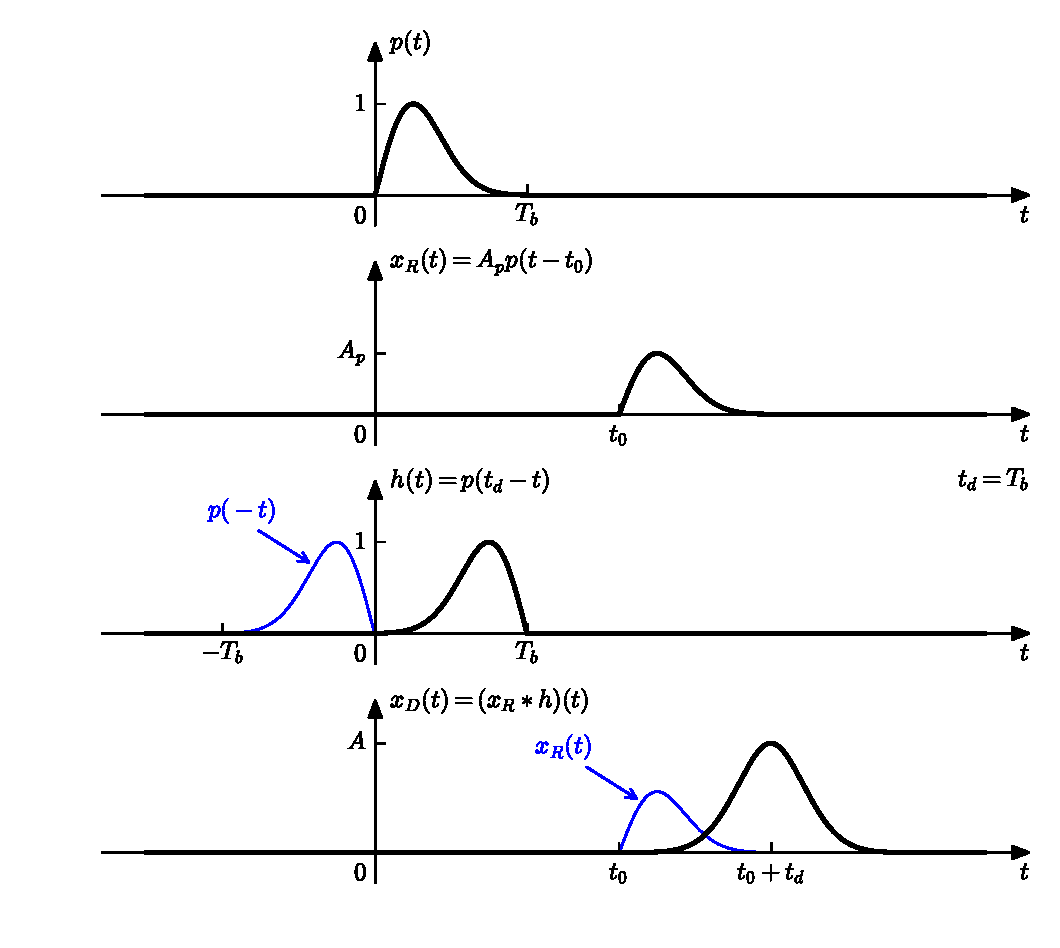
\includegraphics[width=0.9\columnwidth]{figuras/matched_filter_waveforms.eps}
\caption{\label{fig:matched_filter_waveforms} Formas de onda involucradas en el funcionamiento del filtro acoplado. El pulso conformador \(p(t)\) es de duración \(T_b\) y forma arbitraria. La señal recibida \(x_R(t)\) es el pulso \(p(t)\) atenuado y retardado \(t_0\) segundos. Como indica la ecuación \ref{eq:matched_filter_white_noise_impulse_response} y se muestra en la figura, la respuesta al impulso \(h(t)\) del filtro acoplado se obtiene invirtiendo temporalmente al pulso \(p(t)\) para obtener \(p(-t)\) y retardando el pulso invertido una cantidad \(t_d\) segundos, elegida por el diseñador, para obtener \(h(t)=p(t_d-t)\). En el caso de la figura, se eligió \(t_d=T_b\). De esta forma, se obtiene el filtro causal que produce el retardo mínimo. La salida del filtro tiene amplitud \(A\) máxima \(t_d\) segundos después de la llegada del pulso, esto es, en el instante de tiempo \(t_0+t_d\). Los instantes en donde la salida del filtro alcanza amplitud \(A\) son indicadores de la llegada de un pulso.}
\end{center}
\end{figure}

En un sistema de comunicaciones digital, el objetivo del receptor es obtener una réplica de la secuencia de bits generada por cierta fuente de información distante. Si el sistema es en banda base, el transmisor codifica la secuencia de bits como una señal modulada por amplitud de pulsos (PAM, \emph{Pulse Amplitude Modulation}) y la envía a través de un canal, donde se introduce ruido. Para decodificar la secuencia de bits a partir de la señal PAM contaminada con ruido, el receptor puede emplear un filtro acoplado de forma de maximizar relación de la amplitud pico a potencia de ruido de cada pulso en la señal PAM. En la figura \ref{fig:matched_filter_operating} se muestra un ejemplo del funcionamiento del filtro acoplado para esta tarea. En el ejemplo, la secuencia de bits está codificada con un código de línea polar sin retorno a cero (NRZ, \emph{non-return-to-zero}). La señal recibida \(y_R(t)\) consiste en la señal PAM original \(x_R(t)\) contaminada con ruido. La señal \(y_D(t)\) obtenida luego del filtro acoplado tiene picos de amplitud máxima cierto tiempo \(t_d\) después de la llegada de cada pulso. Cada pico es de amplitud positiva o negativa en correspondencia con la amplitud del pulso recibido. Muestreando la señal \(y_D(t)\) en los instantes de amplitud máxima (\(t_n=t_0+t_d+nT_b\), donde \(t_0\) es el retardo introducido en el canal y \(T_b\) es el tiempo de bit), el receptor decide si el pulso corresponde a un 1 o a un 0 lógico según si el valor de la muestra es positivo o negativo respectivamente.
\begin{figure}[!htb]
\begin{center}
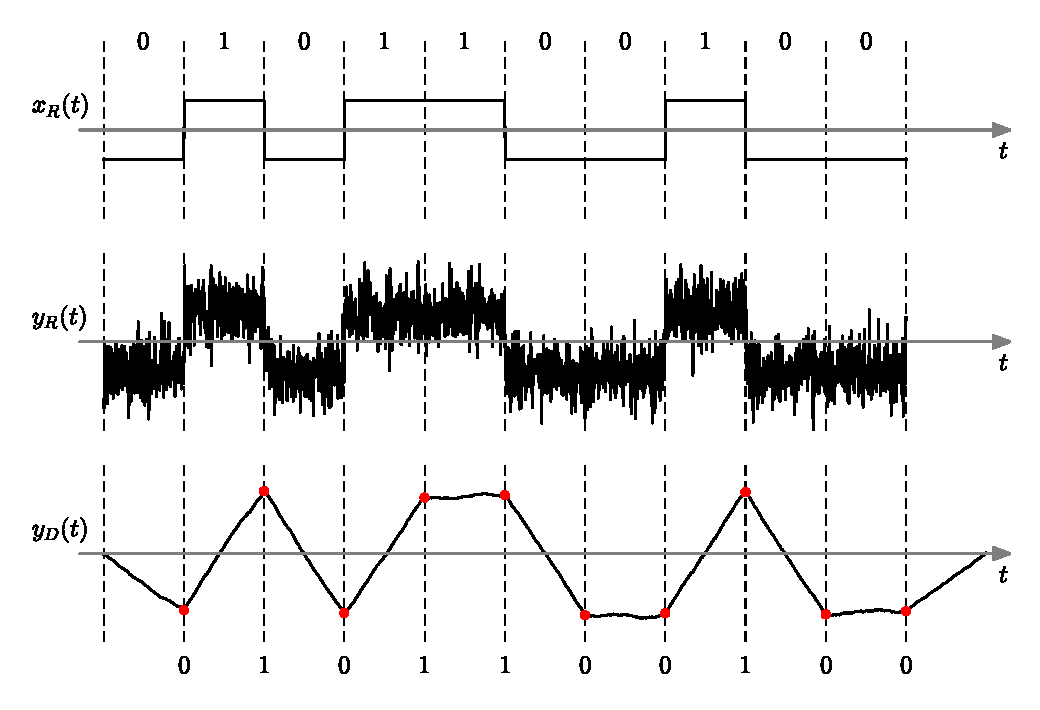
\includegraphics[width=0.9\columnwidth]{figuras/matched_filter_operating.eps}
\caption{\label{fig:matched_filter_operating} Ejemplo de funcionamiento del filtro acoplado. La señal recibida \(y_R(t)\) es una señal PAM digital con código de línea polar sin retorno a cero contaminada por ruido introducido en el canal. El filtro acoplado produce una señal \(y_D(t)\) que tiene picos de amplitud máxima \(t_d\) segundos después de la llegada de cada pulso a la vez que reduce la potencia del ruido. Se eligió el retardo del filtro acoplado \(t_d=T_b\) en este ejemplo. Muestreando \(y_D(t)\) cada \(T_b\) segundos en los instantes de amplitud máxima y evaluando el valor de cada muestra, es posible determinar la polaridad de los pulsos de la señal PAM para decodificar la secuencia de bits.}
\end{center}
\end{figure}

\section{Probabilidad de error con el filtro acoplado}

En esta sección se analiza la probabilidad de error de detección de bits cuando se emplea un filtro acoplado en el receptor. 

En la transmisión de datos digitales en banda base a través de un canal analógico, la secuencia de bits a enviar se codifica como una señal PAM digital de la forma
\begin{equation}\label{eq:digital_pam_waveform}
 x(t)=\sum_{k=-\infty}^{\infty}a_kp(t-kD).
\end{equation}
Como referencia, se considera el caso en donde se emplea un receptor regenerativo que incluye un filtro \textbf{pasabajos ideal}. La probabilidad de error de bits en este caso es (ver capítulo 11 en \cite{Carlson2009})
\begin{equation}\label{eq:generic_error_probability}
 P_e=Q\left(\frac{A}{2\sigma}\right),
\end{equation}
donde \(A\) es la amplitud de la separación entre el nivel bajo y el nivel alto para representar los bits \(0\) y \(1\) respectivamente de la señal PAM recibida, y \(\sigma\) es la desviación estándar del ruido luego del filtro pasabajos. Para la deducción de este resultado se asume que el pasabajos del receptor no introduce interferencia intersimbólica (ISI, \emph{Intersymbol Interference}), el canal no produce distorsión, el ruido introducido en el canal es blanco y gaussiano de media nula y los símbolos \(a_k\) son independientes. Además, se asume que la fuente emite símbolos de forma equiprobable y el receptor emplea el umbral de decisión óptimo.

Si se usa codificación de línea con pulsos \(p(t)\) rectangulares sin retorno a cero, con valores \(a_k\) de \(0\) y \(A\) en el caso unipolar y \(-A/2\) y \(A/2\) en el caso polar para codificar los bits \(0\) y \(1\) respectivamente, la potencia de la señal PAM recibida es
\begin{equation}\label{eq:sr_rectangular_pam}
 S_R=\left\{ 
    \begin{array}{l l l}
    A^2/2 & & \textrm{Unipolar}\\
    A^2/4 & & \textrm{Polar,} \end{array} \right.
\end{equation}
asumiendo que el receptor no produce distorsión significativa y compensa la atenuación del canal, así que se cumple que \(S_R\approx S_x\). Por lo tanto, la probabilidad de error en función de la relación señal a ruido \((S/N)_R\) en predetección, es decir, luego del pasabajos, es
\begin{align*}
  P_e&=Q\left(\frac{A}{2\sigma}\right)
    =\left\{ 
      \begin{array}{l l l}
    Q\left(\sqrt{\frac{1}{2}(S/N)_R}\right) & & \textrm{Unipolar}\\
    Q\left(\sqrt{(S/N)_R}\right) & & \textrm{Polar.} \end{array} \right.
\end{align*}

\subsection{Caso de codificación binaria}\label{sec:error_probability_binary}

Se considera el caso de señalización binaria con un receptor que incluye un filtro acoplado. La señal PAM es de la forma indicada en la ecuación \ref{eq:digital_pam_waveform}, y el pulso conformador \(p(t)\) cumple las condiciones usuales,
\begin{align}
 \begin{split}
 p(0) &= 1  \label{eq:shaped_pulse_centered}\\
 p(t) &= 0, \qquad \textrm{en } |t|>\tau/2,\textrm{ con }\tau\leq D.
 \end{split}
\end{align}
El filtro acoplado en el receptor tiene respuesta al impulso dada por la ecuación  \ref{eq:matched_filter_white_noise_impulse_response}. En particular, se elige la constante \(K\) de forma que la respuesta al impulso sea
\begin{equation}\label{eq:matched_filter_impulse_response}
 h(t)=\frac{1}{\tau_\textrm{eq}}p(t_d-t)
\end{equation}
con
\begin{equation}\label{eq:tau_eq}
  t_d=\tau/2\qquad\qquad\qquad\textrm{y}\qquad\qquad\qquad \tau_\textrm{eq}=\int_{-\infty}^{\infty}p^2(t)\,dt.
\end{equation}
Con \(t_d\) elegido de esta forma, el filtro acoplado es causal con retardo mínimo. La constante de proporcionalidad \(1/\tau_\textrm{eq}\) se eligió de forma que cuando la entrada es un único pulso \(p(t)\) escalado por \(a_k\), \(x(t)=a_kp(t)\), el valor máximo de la salida es \(a_k\). Dicho valor se da en el instante \(t=t_d\). Esta consideración es importante en lo que sigue del razonamiento para calcular la probabilidad de error de bits. Por la deducción de estos resultados, referirse al apéndice \ref{ap:matched_filter_pulse_response_derivation}.

Una señal PAM que cumple las condiciones indicadas arriba, consiste en una sucesión de pulsos donde el pulso \(k\)-ésimo está centrado en el instante \(t_k=kD\), el soporte es el intervalo \([kD-\tau/2,\,kD+\tau/2]\) y está multiplicado por la constante \(a_k\). Notar que debido a que \(\tau\leq D\), los pulsos no se solapan. Como el filtro acoplado es lineal, cuando la entrada es la señal PAM libre de ruido, la salida también es una sucesión de pulsos, donde el pulso \(k\)-ésimo es la respuesta del filtro acoplado al pulso \(k\)-ésimo de la señal PAM de entrada, y por lo tanto, tiene valor máximo \(a_k\) en el instante \(t_k=kD+t_d\) y soporte \([kD+t_d-\tau,\,kD+t_d+\tau]\). Los pulsos en la salida pueden solaparse, ya que el soporte de cada pulso en la salida es de tamaño \(2\tau\), el doble del soporte de los pulsos de la señal PAM de entrada. Sin embargo, no se produce ISI en los instantes \(t_k=kD+t_d\) donde los pulsos toman amplitud máxima. Para ver esto, hay que considerar el caso con mayor solapamiento, que es cuando \(\tau=D\). La respuesta al pulso \(k-1\) se extingue justo en \(kD+t_d\) y la respuesta del pulso \(k+1\) comienza justo \(kD+t_d\), por lo que no interfieren en el valor de la respuesta al pulso \(k\)-ésimo en \(t_k=kD+t_d\). 

Para analizar la probabilidad de error de detección de bits, se considera el caso mas general en que el pulso conformador es de forma \(p(t)\) arbitraria con amplitud máxima unitaria. En la señal PAM unipolar, los pulsos se escalan con \(a_k=\lbrace 0,\,A\rbrace\) para representar el 0 y el 1 lógico respectivamente. Análogamente, en la señal PAM polar los pulsos se escalan con \(a_k=\lbrace -A/2,\,A/2\rbrace\). De esta forma, la diferencia de amplitud máxima entre la representación del 0 y el 1 lógico es \(A\) en ambos casos. Debido a la constante de proporcionalidad \(1/\tau_\textrm{eq}\) en la respuesta \(h(t)\) del filtro acoplado, la diferencia de amplitud máxima de la salida también es \(A\). Esto se ilustra en la figura \ref{fig:matched_filter_pam_output}, donde se muestra un ejemplo de la salida del filtro acoplado cuando la entrada es una señal PAM digital con codificación unipolar y polar. 
Por otro lado, la señal PAM digital llega al receptor contaminada con ruido blanco, que se asume gaussiano y de media nula. Como el filtro acoplado es lineal, el ruido luego del filtro acoplado también es gaussiano y de media nula. Por una demostración de esto, ver por ejemplo la sección 4.4 de \cite{Proakis2001}. Debido a estas dos consideraciones, es decir, que la diferencia de amplitud entre el nivel alto y el bajo de la señal PAM es \(A\), y que el ruido filtrado es gaussiano, la ecuación \ref{eq:generic_error_probability} también es válida para el cálculo de la probabilidad de error de bits cuando el receptor es un filtro acoplado.

\begin{figure}[!htb]
\begin{center}
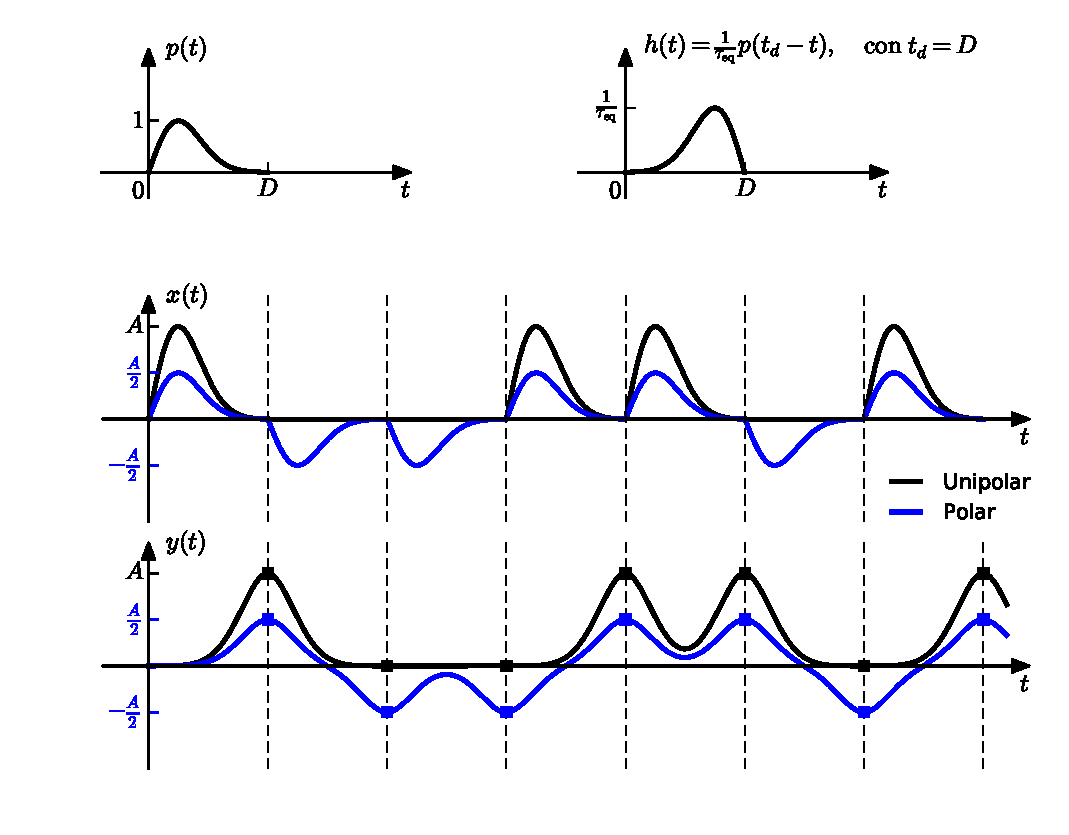
\includegraphics[width=0.9\columnwidth]{figuras/matched_filter_pam_output.eps}
\caption{\label{fig:matched_filter_pam_output} Salida del filtro acoplado cuando la entrada es una señal PAM digital con pulso conformador de forma de onda arbitraria. Arriba en la figura, se muestra la forma de onda del pulso conformador \(p(t)\) y la correspondiente respuesta al impulso del filtro acoplado \(h(t)\). El soporte del pulso conformador es todo el tiempo de pulso, es decir, el intervalo \([0,\,D)\), lo que implica que \(\tau=D\) en este ejemplo. Nótese que, por claridad de la figura, esto es distinto a lo indicado en la sección \ref{sec:error_probability_binary}, en donde el análisis se realizó considerando que el soporte de \(p(t)\) es el intervalo \([-D/2,\,D/2)\). Ahora, hay que eligir \(t_d=D\) de forma que el filtro acoplado sea causal y de retardo mínimo. La señal \(x(t)\) es la señal PAM digital obtenida al codificar la secuencia binaria \texttt{1001101}, usando tanto codificación unipolar (negro) como codificación polar (azul), donde \(a_k=\lbrace 0,\,A\rbrace\) y \(a_k=\lbrace -A/2,\,A/2\rbrace\) respectivamente. El soporte del pulso \(k\)-ésimo de la señal PAM es el intervalo \([kD,\,(k+1)D)\). La señal \(y(t)\) es la respuesta del filtro acoplado cuando la entrada es \(x(t)\). El soporte de la respuesta del pulso \(k\)-ésimo es el intervalo \([kD,\,(k+2)D)\) y el instante de muestreo óptimo es \(t_k=(k+1)D\), donde la amplitud de la salida del filtro acoplado es máxima. Si bien en la salida los pulsos se solapan, en los instantes de muestreo óptimos no se produce ISI. Observar que como la diferencia entre el nivel alto y el nivel bajo máximo en la señal PAM es \(A\) en ambos codificaciones, la diferencia de amplitud entre el nivel alto y el nivel bajo en los instantes de muestreo óptimos también es \(A\) en la salida.}
\end{center}
\end{figure}

Considérese el caso en que el sistema de transmisión tiene una tasa de bits de \(r_b\) bits/s, la potencia de la señal recibida es \(S_R\) W y la densidad del ruido es \(N_0\) W/Hz. Se expresará la probabilidad de error de bits en función de estos parámetros. Como se explica en el apéndice \ref{ap:pam_signal_power}, la potencia de una señal PAM digital es
\[
 S_x=\frac{\overline{a_k^2}}{D}\int_{-\infty}^{\infty}p^2(t)\,dt.
\]
Si el receptor compensa la atenuación del canal y el canal no distorsiona significativamente la señal, \(S_R\approx S_x\). Además, considerando la definición de \(\tau_\textrm{eq}\) dada en la ecuación \ref{eq:tau_eq} y teniendo en cuenta que \(r_b=1/D\), la potencia de la señal recibida es
\begin{equation}\label{eq:sr_generic_pam}
 S_R=\overline{a_k^2}\tau_\textrm{eq}r_b.
\end{equation}
Asumiendo que la fuente binaria emite símbolos de forma equiprobable y que \(a_k=\lbrace 0,\,A\rbrace\) y \(a_k=\lbrace -A/2,\,A/2\rbrace\) en el caso unipolar y polar respectivamente,
\[
\overline{a_k^2}=\left\{ 
    \begin{array}{l l l l l}
    \dfrac{1}{2}\times0^2+\dfrac{1}{2}\times A^2 & = & \dfrac{A^2}{2} & & \textrm{Unipolar}\\
    \\
    \dfrac{1}{2}\times\left(-\dfrac{A}{2}\right)^2+\dfrac{1}{2}\times\left(\dfrac{A}{2}\right)^2 & = & \dfrac{A^2}{4} & & \textrm{Polar,} \end{array} \right.
\]
y por lo tanto,
\[
S_R=\left\{ 
    \begin{array}{l l l}
    \dfrac{A^2\tau_\textrm{eq}r_b}{2} & & \textrm{Unipolar}\\
    \\
    \dfrac{A^2\tau_\textrm{eq}r_b}{4} & & \textrm{Polar.} \end{array} \right.
\]
En el caso particular en que el pulso conformador \(p(t)\) es rectangular, \(\tau_\textrm{eq}=D=1/r_b\), y el resultado coincide con el de la ecuación \ref{eq:sr_rectangular_pam}. Despejando \(A\) se llega a que
\begin{equation}\label{eq:pma_amplitude_vs_sr}
 A=\left\{ 
    \begin{array}{l l l}
    \sqrt{\dfrac{2S_R}{\tau_\textrm{eq}r_b}} & & \textrm{Unipolar}\\
    \\
    \sqrt{\dfrac{4S_R}{\tau_\textrm{eq}r_b}} & & \textrm{Polar.} \end{array} \right.
\end{equation}

Para el cálculo de la probabilidad de error también hay que calcular la potencia del ruido \(N_R\) en predetención. Si el ruido contaminante es blanco con PSD \(G_{n_R}(f)=N_0/2\), la potencia del ruido a la salida del filtro acoplado es
\begin{align*}
 N_{R}=\sigma^2&=\int_{-\infty}^{\infty}\left|H(f)\right|^2G_{n_R}(f)\,df\\
  &=\frac{N_0}{2}\int_{-\infty}^{\infty}\left|H(f)\right|^2\,df\\
  &\overset{(a)}{=}\frac{N_0}{2}\int_{-\infty}^{\infty}\left|h(t)\right|^2\,dt\\
  &\overset{(b)}{=}\frac{N_0}{2\tau_\textrm{eq}^2}\int_{-\infty}^{\infty}\left|p(t_d-t)\right|^2\,dt\\
  &\overset{(c)}{=}\frac{N_0}{2\tau_\textrm{eq}^2}\int_{-\infty}^{\infty}\left|p(u)\right|^2\,du,
\end{align*}
donde en \((a)\) se empleó la identidad de Parseval, en \((b)\) se sustituyó \(h(t)\) usando la ecuación \ref{eq:matched_filter_impulse_response} y en \((c)\) se realizó el cambio de variable \(u=t_d-t\). Finalmente, usando la ecuación \ref{eq:tau_eq} se obtiene que
\[
 N_{R}=\sigma^2=\frac{N_0}{2\tau_\textrm{eq}},
\]
es decir,
\begin{equation}\label{eq:matched_filter_nr}
 \sigma=\sqrt{\frac{N_0}{2\tau_\textrm{eq}}}.
\end{equation}
Usando las ecuaciones \ref{eq:pma_amplitude_vs_sr} y \ref{eq:matched_filter_nr} se tiene que, por ejemplo, para el caso unipolar,
\[
 \frac{A}{2\sigma}=\frac{\sqrt{\dfrac{2S_R}{\tau_\textrm{eq}r_b}}}{2\sqrt{\dfrac{N_0}{2\tau_\textrm{eq}}}}
 =\sqrt{\dfrac{S_R}{N_0r_b}},
\]
por lo tanto, la probabilidad de error resulta en
\begin{equation*}
 P_e=Q\left(\frac{A}{2\sigma}\right)
    =\left\{ 
      \begin{array}{l l l}
    Q\left(\sqrt{\dfrac{S_R}{N_0r_b}}\right) & & \textrm{Unipolar}\\
    \\
    Q\left(\sqrt{\dfrac{2S_R}{N_0r_b}}\right) & & \textrm{Polar.} \end{array} \right.
\end{equation*}

Para caracterizar el sistema de transmisión, se definen dos nuevos parámetros, \(E_b\) y \(\gamma_b\), de la siguiente forma,
\begin{align*}
 E_b &= \frac{S_R}{r_b}\\
 \gamma_b &= \frac{E_b}{N_0}.
\end{align*}
 \(E_b\) es la \emph{energía promedio por bit} y \(\gamma_b\) es la \emph{energía promedio por bit normalizada}, que consiste en la razón entre la energía promedio por bit y la densidad de ruido. La probabilidad de error se puede expresar en función de estos parámetros como
\begin{equation*}
 P_e=\left\{ 
      \begin{array}{l l l}
    Q\left(\sqrt{\dfrac{E_b}{N_0}}\right) & & \textrm{Unipolar}\\
    \\
    Q\left(\sqrt{\dfrac{2E_b}{N_0}}\right) & & \textrm{Polar.} \end{array} \right.
\end{equation*}
o
\begin{equation*}
 P_e=\left\{ 
      \begin{array}{l l l}
    Q\left(\sqrt{\gamma_b}\right) & & \textrm{Unipolar}\\
    \\
    Q\left(\sqrt{2\gamma_b}\right) & & \textrm{Polar.} \end{array} \right.
\end{equation*}

\subsubsection*{Resumen y conclusiones}

La probabilidad de error de bits es función del cociente \(A/(2\sigma)\), tanto si el receptor incluye un filtro pasabajos o un filtro acoplado como el definido por la ecuación \ref{eq:matched_filter_impulse_response}. \(A\) es la diferencia de amplitud en los instantes de muestreo óptimos entre las representaciones del 0 y el 1 lógico en la señal PAM filtrada.
Para ambos filtros, el pasabajos y el acoplado, la amplitud \(A\) se puede expresar en función de los parámetros del sistema como se indica en la siguiente tabla:
\begin{center}
\begin{tabular}{l c c}
& Pulso rectangular & Pulso arbitrario \\  
\\
Unipolar & \(A=\sqrt{2S_R}\)  &  \(A=\sqrt{\dfrac{2S_R}{\tau_\textrm{eq}r_b}}\) \\
Polar & \(A=\sqrt{4S_R}\)  &  \(A=\sqrt{\dfrac{4S_R}{\tau_\textrm{eq}r_b}}\) \\
\end{tabular}
\end{center}

La potencia del ruido filtrado, \(N_R=\sigma^2\), depende del tipo de filtro empleado. Si en el receptor hay un filtro pasabajos, la potencia del ruido filtrado es
\[
 N_R=N_0B_N,
\]
donde \(B_N\) es la frecuencia de corte del pasabajos. Notar que la potencia del ruido decrece al reducir el ancho de banda \(B_N\) del filtro pasabajos. Sin embargo, éste no puede hacerse arbitrariamente pequeño debido a la limitación de la tasa de Nyquist, que indica que
\[
 B_N\geq\frac{r_b}{2}.
\]
Si esto no se cumpliera, la señal sería severamente distorsionada por el filtro pasabajos, produciendo interferencia intersimbólica que haría imposible la detección de bits. Por lo tanto, al emplear un pasabajos, la potencia del ruido está acotada inferiormente como
\begin{equation}\label{eq:noise_power_lower_bound}
 N_R\geq\frac{N_0r_b}{2}.
\end{equation}
Si en el receptor hay un filtro acoplado, la potencia del ruido filtrado es
\[
 N_R=\frac{N_0}{2\tau_\textrm{eq}},
\]
y se cumple que \(\tau_\textrm{eq}\leq D=1/r_b\), donde la igualdad se da cuando el pulso conformador es rectangular, ya que en ese caso
\[
 \tau_\textrm{eq}=\int_{-\infty}^{\infty}p^2(t)\,dt=\int_{0}^{D}1^2\,dt=t\,\bigg|_{0}^D=D.
\]
Esto indica que en el caso del filtro acoplado, la potencia del ruido también está acotado inferiormente por la ecuación \ref{eq:noise_power_lower_bound} y la igualdad se da si el pulso conformador es rectangular. En este caso, se alcanza el criterio de la tasa de Nyquist sin que se produzca ISI en los instantes de muestreo óptimos.

\subsection{Caso de codificación \emph{M}-aria}

A continuación se deduce la probabilidad de error de bits en el caso de señalización \(M\)-aria. Una señal \(M\)-aria posee \(M>2\) niveles de amplitud, por lo que la separación entre niveles es mas pequeña que la separación entre niveles de una señal binaria de la misma potencia. Por lo tanto, para una relación señal a ruido fija, la señalización \(M\)-aria es mas sensible al ruido debido a que es mas probable confundir entre niveles. Por otro lado, para una velocidad de transmisión de bits fija, la tasa de señalización de la señal \(M\)-aria es menor que la tasa de bits de la señal binaria equivalente. Esto significa que la codificación \(M\)-aria requiere menor ancho de banda. En conclusión, la codificación \(M\)-aria es apropiada en aplicaciones donde el ancho de banda es limitado y la relación señal a ruido es relativamente grande.

Para el cálculo de la probabilidad de error \(M\)-aria se asume como antes que el ruido contaminante es blanco, gaussiano y de media nula. Se considera el caso en que las amplitudes de los niveles de la señal \(M\)-aria son
\begin{equation}\label{eq:m-ary_ak}
 a_k=\pm \frac{A}{2},\,\pm \frac{3A}{2},\,\dots,\,\pm \frac{(M-1)A}{2},
\end{equation}
por lo que la señalización es polar, y el número de niveles es par y están equiespaciados una magnitud \(A\). La probabilidad de error de detección promedio de un símbolo es
\begin{equation}\label{eq:generic_m-ary_error_probability}
 P_e = \sum_{i=0}^{M-1}P_iP_{e_i},
\end{equation}
donde \(P_i\) es la probabilidad de emisión del símbolo \(i\)-ésimo de la fuente y \(P_{e_i}\) es la probabilidad de error de detección del símbolo \(i\)-ésimo, con \(i=0,\,\dots,\,M-1\). Se asume además que la fuente emite símbolos de forma equiprobable, por lo que \(P_i=1/M\) para todo \(i\) y la ecuación \ref{eq:generic_m-ary_error_probability} se reduce a
\begin{equation}\label{eq:generic_m-ary_error_probability_aux}
 P_e = \frac{1}{M}\sum_{i=0}^{M-1}P_{e_i}.
\end{equation}

En la figura \ref{fig:quaternary_gaussian_noise} se muestran las densidades de probabilidad condicional de la amplitud correspondiente a cada símbolo para una señal polar cuaternaria, es decir, con \(M=4\), contaminada con ruido gaussiano. En este caso, los cuatro niveles de amplitud de la señal limpia son \(a_k=\pm A/2,\,\pm 3A/2\), y hay tres umbrales de decisión óptimos para minimizar \(P_e\), que son \(-A\) , 0 y \(A\). Sin embargo, a diferencia del caso binario, la probabilidad de error de detección \(P_{e_i}\) no es igual para todos los símbolos. Como se observa en la figura, los símbolos de los extremos, representados con la amplitud mínima y máxima de la señal PAM cuaternaria, tienen probabilidad de error de detección
\[
 P_{e_0}=P_{e_3}=Q\left(\frac{A}{2\sigma}\right),
\]
mientras que la probabilidad de error de detección de los niveles intermedios es
\[
 P_{e_1}=P_{e_2}=2Q\left(\frac{A}{2\sigma}\right),
\]
ya que en este caso, es posible confundir el símbolo con los dos símbolos adyacentes. Por lo tanto, usando la ecuación \ref{eq:generic_m-ary_error_probability_aux}, la probabilidad de error promedio es
\begin{align*}
 P_e&=\frac{1}{4}\times6Q\left(\frac{A}{2\sigma}\right)\\
    &=\frac{3}{2}Q\left(\frac{A}{2\sigma}\right),
\end{align*}
es decir, un 50\% mayor que la señalización binaria con la misma diferencia de amplitud entre niveles (ver ecuación \ref{eq:generic_error_probability}).
\begin{figure}[!htb]
\begin{center}
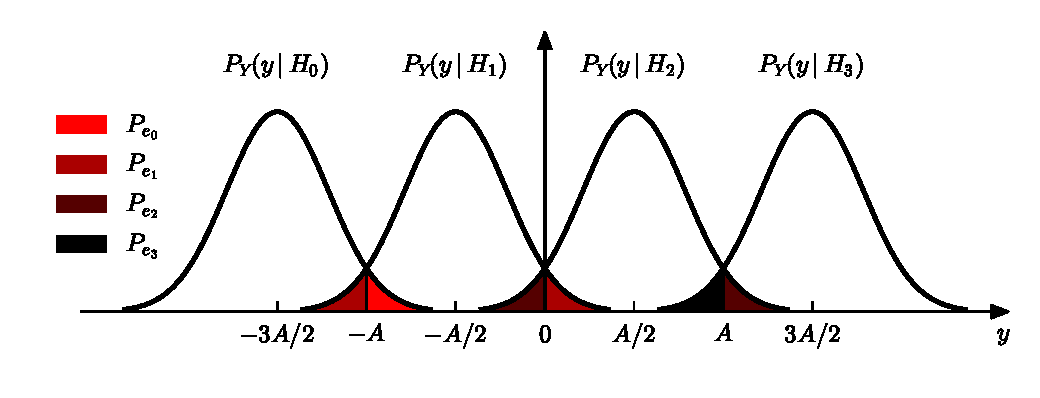
\includegraphics[width=0.9\columnwidth]{figuras/quaternary_gaussian_noise.eps}
\caption{\label{fig:quaternary_gaussian_noise} Densidad de probabilidad condicional de cada nivel de amplitud de una señal polar cuaternaria contaminada con ruido blanco gaussiano de varianza \(\sigma^2\).  La probabilidad de error de los niveles de amplitud de los extremos es \(P_{e_0}=P_{e_3}=Q(A/2\sigma)\), mientras que la de los niveles de amplitud intermedios es \(P_{e_1}=P_{e_2}=2Q(A/2\sigma)\), el doble que la de los símbolos de los extremos.}
\end{center}
\end{figure}

Para un valor arbitrario de \(M\), hay \(M-1\) umbrales de decisión óptimos en 
\[
 y = 0,\,\pm A,\,\pm2A,\,\dots,\pm\frac{M-2}{2}A.
\]
Como se explicó antes, la probabilidad de error de detección de los \(M-2\) niveles intermedios es el doble que la de los dos niveles extremos, que es \(P_{e_0}=P_{e_{M-1}}=Q\left(A/2\sigma\right)\). Por lo tanto, la probabilidad promedio de error es
\begin{align*}
  P_e &= \frac{1}{M}\left[2Q\left(\frac{A}{2\sigma}\right)+(M-2)2Q\left(\frac{A}{2\sigma}\right)\right]\\
      &=\frac{2(M-1)}{M}Q\left(\frac{A}{2\sigma}\right),
\end{align*}
resultando en
\begin{equation}\label{eq:m-ary_error_probability}
  P_e=2\left(1-\frac{1}{M}\right)Q\left(\frac{A}{2\sigma}\right).
\end{equation}
Como es de esperar, en el caso binario la ecuación \ref{eq:m-ary_error_probability} coincide con la ecuación \ref{eq:generic_error_probability}, mientras que \(P_e\) tiende a duplicarse a medida que se incrementa \(M\), ya que \(P_e\approx 2Q\left(A/2\sigma\right)\) si \(M\gg 2\).

Al igual que en el caso binario, es de interés expresar la probabilidad de error en función de la potencia de la señal y la densidad del ruido. Como indica la ecuación \ref{eq:sr_generic_pam}, la potencia de la señal PAM recibida es
\[
 S_R=\overline{a_k^2}\tau_\textrm{eq}r,
\]
donde \(r\) es la tasa de símbolos \(M\)-arios y \(\tau_\textrm{eq}\) está definido por la ecuación \ref{eq:tau_eq}. Teniendo en cuenta que
\[
 \overline{a_k^2}=A^2\frac{(M^2-1)}{12},
\]
como se muestra en al apéndice \ref{ap:m-ary_ak_square_mean}, la potencia se puede expresar en función de la amplitud como,
\[
 A^2=\frac{12}{M^2-1}\,\frac{S_R}{\tau_\textrm{eq}r},
\]
y por lo tanto
\begin{equation}\label{eq:m-ary_amplitude_to_noise}
 \left(\frac{A}{2\sigma}\right)^2=\frac{3}{M^2-1}\,\frac{1}{\tau_\textrm{eq}r}\,\frac{S_R}{N_R},
\end{equation}
donde \(N_R=\sigma^2\) es la potencia del ruido filtrado. Si se emplea un filtro acoplado en el receptor, se cumple que \(N_{R}=N_0/2\tau_\textrm{eq}\) (ecuación \ref{eq:matched_filter_nr_2}) y entonces
\begin{equation}\label{eq:m-ary_amplitude_to_noise_rectangular}
 \left(\frac{A}{2\sigma}\right)^2=\frac{6}{M^2-1}\,\frac{S_R}{N_0r},
\end{equation}
y la probabilidad de error queda
\begin{equation}\label{eq:m-ary_error_probability_matched_filter}
 P_e=2\left(1-\frac{1}{M}\right)Q\left(\sqrt{\frac{6}{M^2-1}\,\frac{S_R}{N_0r}}\right),
\end{equation}
que se podría expresar en función de la energía promedio por símbolo \(M\)-ario \(E_M=S_R/r\).
Notar que si el código de línea usa pulsos rectangulares NRZ, \(\tau_\textrm{eq}=D=1/r\), y a partir de las ecuaciones \ref{eq:m-ary_error_probability} y \ref{eq:m-ary_amplitude_to_noise}, se obtiene que la probabilidad de error es
\[
 P_e=2\left(1-\frac{1}{M}\right)Q\left(\sqrt{\frac{3}{M^2-1}\,\frac{S_R}{N_R}}\right).
\]

La ecuación \ref{eq:m-ary_error_probability_matched_filter} indica la probabilidad de error promedio de un símbolo \(M\)-ario con codificación polar cuando el receptor incluye un filtro acoplado. 
Normalmente, se usa codificación \(M\)-aria para representar mensajes binarios. En estos casos, es de mayor utilidad obtener una expresión de la probabilidad de error de bits del sistema, en lugar del error de símbolos \(M\)-arios. De forma acorde, en un sistema de transmisión binario, uno de los parámetros de interés es la tasa de bits \(r_b\), y no la tasa de símbolos \(M\)-arios \(r\), de la cual es función la ecuación \ref{eq:m-ary_error_probability_matched_filter}. 

Si la codificación \(M\)-aria se usa para la transmisión de mensajes binarios, donde cada nivel \(M\)-ario representa una palabra de longitud \(\log_2M\) bits, \(r_b\) se relaciona con \(r\) como
\begin{equation}\label{eq:r_b_vs_r}
 r_b=r\log_2M.
\end{equation}
Para definir la probabilidad de error de bits que producen los errores de símbolos \(M\)-arios, es necesario establecer algunas hipótesis. Se asumirá que los niveles \(M\)-arios representan palabras binarias de un código Grey, y por lo tanto, dos niveles sucesivos representan palabras binarias que difieren solo en un bit. También se asumirá que la relación señal a ruido es relativamente grande, de forma que es poco probable que la amplitud del ruido supere mas de un nivel de la señal \(M\)-aria. Ambas hipótesis implican que un símbolo \(M\)-ario detectado erróneamente difiere solo en un nivel del símbolo correcto y ésto corresponde a un único bit erróneo en la palabra de \(\log_2M\) bits. Por lo tanto,
\[
 P_{be}\approx\frac{P_e}{\log_2M},
\]
donde \(P_{be}\) es la probabilidad de error de bits equivalente, también denominada \textbf{tasa de error de bits} (BER, \emph{Bit Error Rate}). Sustituyendo estos resultados en las ecuaciones \ref{eq:m-ary_error_probability} y \ref{eq:m-ary_amplitude_to_noise_rectangular}, se obtiene que
\begin{equation}\label{eq:m-ary_bit_error_error_probability}
 P_{be}=2\,\frac{M-1}{M\log_2M}\,Q\left(\frac{A}{2\sigma}\right)
\end{equation}
si el código de línea usa pulsos rectangulares NRZ, donde 
\begin{align}\label{eq:m-ary_amplitude_to_noise_aux}
 \left(\frac{A}{2\sigma}\right)^2&\leq\frac{6\log_2M}{M^2-1}\,\frac{S_R}{N_0r_b}\nonumber\\ 
   &=\frac{6\log_2M}{M^2-1}\,\gamma_b,
\end{align}
y la igualdad se alcanza si se emplea un filtro acoplado. En la última ecuación se expresó el resultado en función de la energía promedio por bit normalizada \(\gamma_b\).

\subsubsection*{Resumen}

En el caso de señalización \(M\)-aria polar con separación entre niveles de amplitud \(A\) y ruido contaminante blanco gaussiano, la probabilidad de error está dada por la ecuación \ref{eq:m-ary_error_probability}
\[
  P_e=2\left(1-\frac{1}{M}\right)Q\left(\frac{A}{2\sigma}\right),
\]
donde en el caso mas general, para una forma de pulso conformador arbitraria e independientemente del filtro en el receptor,
\[
 \left(\frac{A}{2\sigma}\right)^2=\frac{3}{M^2-1}\,\frac{1}{\tau_\textrm{eq}r}\,\frac{S_R}{N_R},
\]
como indica la ecuación \ref{eq:m-ary_amplitude_to_noise}, donde \(\sigma^2=N_R\) es la potencia del ruido luego del filtro del receptor. Si el pulso conformador es rectangular NRZ, \(\tau_\textrm{eq}r=1\), y por lo tanto la ecuación \ref{eq:m-ary_amplitude_to_noise} se reduce a
\[
 \left(\frac{A}{2\sigma}\right)^2=\frac{3}{M^2-1}\,\frac{S_R}{N_R}.
\]

En el caso en que se emplee un filtro acoplado en el receptor, se cumple que \(N_{R}=N_0/2\tau_\textrm{eq}\), y la ecuación \ref{eq:m-ary_amplitude_to_noise} queda
\[
 \left(\frac{A}{2\sigma}\right)^2=\frac{6}{M^2-1}\,\frac{S_R}{N_0r},
\]
independientemente de la forma del pulso conformador, y donde \(N_0\) es la densidad del ruido blanco contaminante.


\subsection{Comparación entre señalización binaria y \emph{M}-aria}

La elección de \(M\) involucra diversos compromisos. Por un lado, para una tasa de símbolos \(r\) fija, el incremento de \(M\) permite la transmisión de una tasa de bits \(r_b\) mas alta (ecuación \ref{eq:r_b_vs_r}). Por otro lado, si se mantiene fija la tasa de bits, el incremento de \(M\) permite la transmisión a una tasa de símbolos \(r\) mas lenta, lo que implica menor ancho de banda de transmisión. Pero si se mantiene la potencia de la señal fija, crece la probabilidad de error al incrementar \(M\), ya que los niveles de la señal \(M\)-aria están mas juntos haciendo que \(A/2\sigma\) decrezca. Por lo tanto, para mantener constante la probabilidad de error es necesario incrementar la potencia de la señal al incrementar \(M\).

Para ilustrar estos compromisos se considera el siguiente ejemplo. Sea un canal por el que se transmite a una tasa de señalización fija de \(r=3000\) baudios (3 kbaudios) y se mantiene fija la potencia de la señal, resultando en una relación señal a ruido de \((S/N)_R=400\approx26\) dB. Se asume que la señalización usa pulsos rectangulares NRZ y el receptor incluye un filtro acoplado, por lo que se cumple que (ecuaciones \ref{eq:m-ary_bit_error_error_probability}, \ref{eq:m-ary_amplitude_to_noise} con \(\tau_\textrm{eq}r=1\) y \ref{eq:m-ary_amplitude_to_noise_aux})
\[
 P_{be}=2\,\frac{M-1}{M\log_2M}\,Q\left(\frac{A}{2\sigma}\right),\qquad\textrm{con}\qquad \left(\frac{A}{2\sigma}\right)^2=\frac{3}{M^2-1}\frac{S_R}{N_R}=\frac{6\log_2M}{M^2-1}\,\gamma_b.
\]
En la tabla a continuación se muestra el incremento en la tasa de bits y el deterioro de la probabilidad de error de bits al incrementar \(M\).
\begin{center}
\bgroup
\def\arraystretch{1.2}
\begin{tabular}{c c S c}\hline
\boldmath\(M\) & \boldmath\(r_b\) (kbps) & \boldmath\(A/2\sigma\) & \boldmath\(P_{be}\) \\\hline
2 & 3  &  20.0 & \(3\times10^{-89}\) \\
4 & 6  &  8.9 & \(1\times10^{-19}\) \\
8 & 9  &  4.4 & \(4\times10^{-6}\) \\
16 & 12  &  2.2 & \(7\times10^{-3}\) \\
32 & 15  &  1.1 & \(6\times10^{-2}\)\\\hline
\end{tabular}
\egroup
\end{center}

Supóngase ahora que se desea transmitir a una tasa de bits \(r_b=9\) kbps fija y además, mantener la probabilidad de error de bits \(P_{be}=4\times10^{-6}\) constante. Si se incrementa \(M\), la tasa de señalización decrece, reduciendo el ancho de banda de transmisión, pero simultáneamente, la potencia de la señal debe incrementarse para mantener la separación entre los niveles de la señal \(M\)-aria y así no cambiar la probabilidad de error. Los resultados se muestran en la siguiente tabla.
\begin{center}
\bgroup
\def\arraystretch{1.2}
\begin{tabular}{c S S}\hline
\boldmath\(M\) & \boldmath\(r\) (kbaudios) & \boldmath\(\gamma_b\) \\\hline
2 & 9  &  10.0  \\
4 & 4.5  &  24.2  \\
8 & 3  &  66.2  \\
16 & 2.25  &  196.5  \\
32 & 1.8  &  618.2 \\\hline
\end{tabular}
\egroup
\end{center}
En la tabla, el valor de \(\gamma_b\) se obtiene despejando de las ecuaciones \ref{eq:m-ary_bit_error_error_probability} y \ref{eq:m-ary_amplitude_to_noise_aux}, y es
\[
 \gamma_b = \frac{M^2-1}{6\log_2M}\left[Q^{-1}\left(\frac{M\log_2M}{2\left(M-1\right)}\,P_{be}\right)\right]^2.
\]


% 
\vspace{1cm}
TODO:
\begin{enumerate}
 \item Implementación con integrador.
 \item Ver el Lathi sobre el comentario de que la configuración filtro acoplado y muestreador es óptima.
\end{enumerate}


\newpage

\appendix

\section{Respuesta al impulso del filtro acoplado}\label{ap:matched_filter_impulse_response_derivation}

Para obtener la respuesta al impulso del filtro acoplado de la ecuación \ref{eq:matched_filter_white_noise_impulse_response} hay que aplicar la antitranformada de Fourier a la ecuación \ref{eq:matched_filter_white_noise_transfer_function}. El resultado es directo si se consideran las siguientes propiedades de la transformada de Fourier. Si \(p(t)\) y \(P(f)\) son un par de transformadas de Fourier, es decir,
\[
 p(t)\overset{\mathcal{F}}{\longleftrightarrow}P(f),
\]
 se cumple que,
\[
 p^*(-t)\overset{\mathcal{F}}{\longleftrightarrow}P^*(f),
\]
y que
\[
 p(t-t_d)\overset{\mathcal{F}}{\longleftrightarrow}P(f)e^{-j2\pi ft_d}.
\]
Combinando ambas propiedades, se deduce que
\[
 p^*(t_d-t)\overset{\mathcal{F}}{\longleftrightarrow}P^*(f)e^{-j2\pi ft}.
\]

Otra forma de obtener el mismo resultado es mediante el cálculo explícito de la antitransformada de Fourier de la función de transferencia de la ecuación \ref{eq:matched_filter_white_noise_transfer_function}. Teniendo en cuenta que \(p(t)\) y \(P(f)\) son un par de transformadas de Fourier, se cumple que,
\begin{equation}\label{eq:inverse_fourier_transform_definition}
 p(t)=\int_{-\infty}^{\infty}P(f)e^{j2\pi ft}\,df.
\end{equation}
Aplicando la transformada inversa de Fourier a la ecuación \ref{eq:matched_filter_white_noise_transfer_function} y operando, se ve que\footnote{Se omite la constante multiplicativa por claridad.}
\begin{align*}
 \mathcal{F}^{-1}\left[P^*(f)e^{-j2\pi ft_d}\right]&\overset{(a)}{=}\int_{-\infty}^{\infty}P^*(f)e^{-j2\pi ft_d}e^{j2\pi ft}\,df\\
 &=\int_{-\infty}^{\infty}P^*(f)e^{-j2\pi f(t_d-t)}\,df\\
 &\overset{(b)}{=}\left(\int_{-\infty}^{\infty}P(f)e^{j2\pi f(t_d-t)}\,df\right)^*\\
 &\overset{(c)}{=}p^*(t_d-t),
\end{align*}
donde en \((a)\) se empleó la definición de la antitranformada de Fourier, en \((b)\) se conjugó la integral y su argumento manteniendo la igualdad y en \((c)\) se observó que la integral entre paréntesis es la ecuación \ref{eq:inverse_fourier_transform_definition} evaluada en \(t_d-t\).
 
\section{Respuesta a un pulso del filtro acoplado}\label{ap:matched_filter_pulse_response_derivation}

En este apéndice se analizan las características temporales de la respuesta a un pulso del filtro acoplado. Sea la entrada \(x(t)=a_kp(t)\), donde \(p(t)\) es un pulso de forma de onda arbitraria que cumple que
\[
\begin{array}{l l l l}
    p(0) & = & 1 &  \\
    p(t) & = & 0 & \quad\textrm{en } |t|>\tau/2,\textrm{ con }\tau\leq D,
\end{array}
\]
y sea el filtro acoplado con respuesta al impulso
\[
 h(t)=\frac{1}{\tau_\textrm{eq}}p(t_d-t)
\]
donde
\[
 \tau_\textrm{eq}=\int_{-\infty}^{\infty}p^2(t)\,dt\qquad\qquad\textrm{y}\qquad\qquad t_d=\tau/2.
\]
La constante de proporcionalidad \(1/\tau_\textrm{eq}\) se eligió de forma tal que cuando la entrada es un pulso \(p(t)\) escalado por \(a_k\), el valor máximo de la salida es \(a_k\).
Para ver esto, considérese la salida \(y(t)\) cuando la entrada es \(x(t)=a_kp(t)\). La salida \(y(t)\) es la convolución entre la entrada \(x(t)\) y la respuesta al impulso \(h(t)\),
\begin{align}\label{eq:matched_filter_pulse_output}
 y(t)&=\left(x*h\right)(t)\nonumber \\
     &=\int_{-\infty}^{\infty}x(u)h(t-u)\,du\nonumber\\
     &=\int_{-\infty}^{\infty}a_kp(u)\frac{1}{\tau_\textrm{eq}}p(t_d-\left[t-u\right])\,du\nonumber\\
     &=\frac{a_k}{\tau_\textrm{eq}}\int_{-\infty}^{\infty}p(u)p(u-\left[t-t_d\right])\,du.
\end{align}
La integral de la ecuación \ref{eq:matched_filter_pulse_output} es una función de \(t\) que toma el valor máximo cuando los dos pulsos del argumento están perfectamente solapados en el tiempo. Esto ocurre cuando \(t=t_d\), y el valor máximo de la salida es
\begin{align*}
 y(t_d)&=\frac{a_k}{\tau_\textrm{eq}}\int_{-\infty}^{\infty}p^2(u)\,du\\
       &=a_k,
\end{align*}
que es lo que se quería mostrar.

Para determinar el soporte temporal de la salida, se observa que la integral de la ecuación \ref{eq:matched_filter_pulse_output} es nula si los soportes de los pulsos del argumento no se solapan.
El soporte de \(p(u)\) es el intervalo \([-\tau/2,\,\tau/2]\) y el soporte de \(p(u-\left[t-t_d\right])\) es el intervalo \([t-t_d-\tau/2,\,t-t_d+\tau/2]\). Por lo tanto, como se muestra en la figura \ref{fig:matched_filter_output_support}, ambos pulsos tienen soportes disjuntos si se cumple que
\[
 t-t_d+\dfrac{\tau}{2} \leq -\dfrac{\tau}{2}\qquad\qquad\textrm{o}\qquad\qquad t-t_d-\dfrac{\tau}{2} \geq  \dfrac{\tau}{2},
\]
es decir, si
\[
 t\leq t_d-\tau\qquad\qquad\textrm{o}\qquad\qquad t \geq  t_d+\tau,
\]
correspondiendo a cuando \(p(u-\left[t-t_d\right])\) está a la izquierda o a la derecha de \(p(t)\) respectivamente. Por lo tanto, el soporte de la salida es el intervalo
\[
 t_d-\tau < t < t_d+\tau.
\]
Finalmente, teniendo en cuenta que se eligió \(t_d=\tau/2\), el soporte temporal de la salida es
\[
 -\frac{\tau}{2} < t < \frac{3\tau}{2},
\]
y el valor máximo se da en el instante \(t=\tau/2\) y es \(a_k\).
\begin{figure}[!htb]
\begin{center}
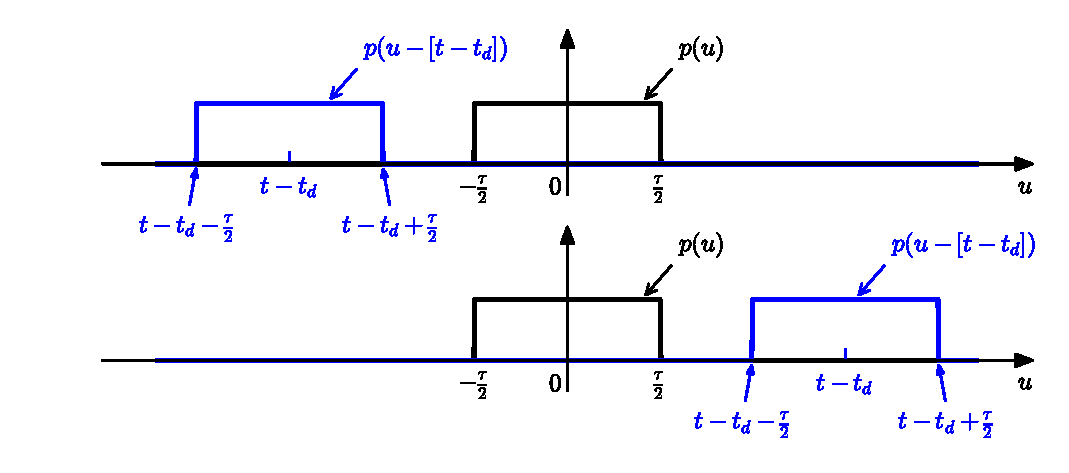
\includegraphics[width=0.9\columnwidth]{figuras/matched_filter_output_support.eps}
\caption{\label{fig:matched_filter_output_support} Deducción del soporte temporal de la respuesta a un pulso del filtro acoplado. En las gráficas, se muestran los pulsos del argumento de la integral de la ecuación \ref{eq:matched_filter_pulse_output}. Cuando los pulsos no se solapan, la respuesta \(y(t)\) es nula. La gráfica superior corresponde al caso en que el valor de \(t\) es tal que el pulso \(p(u-[t-t_d])\) se encuentra a la izquierda de \(p(t)\). Como se evidencia en la gráfica, los pulsos no se solapan si se cumple que \(t-t_d+\tau/2 \leq -\tau/2\). En la gráfica inferior se muestra la situación en que el pulso \(p(u-[t-t_d])\) se encuentra a la derecha de \(p(t)\). En este caso, no hay solapamiento si \(t-t_d-\tau/2 \geq \tau/2\).}
\end{center}
\end{figure}
 
En la figura \ref{fig:matched_filter_square_pulse_output} se muestran las formas de onda involucradas en el cálculo de la respuesta a un pulso \(x(t)=a_kp(t)\) del filtro acoplado cuando el pulso conformador \(p(t)\) es rectangular.
\begin{figure}[!htb]
\begin{center}
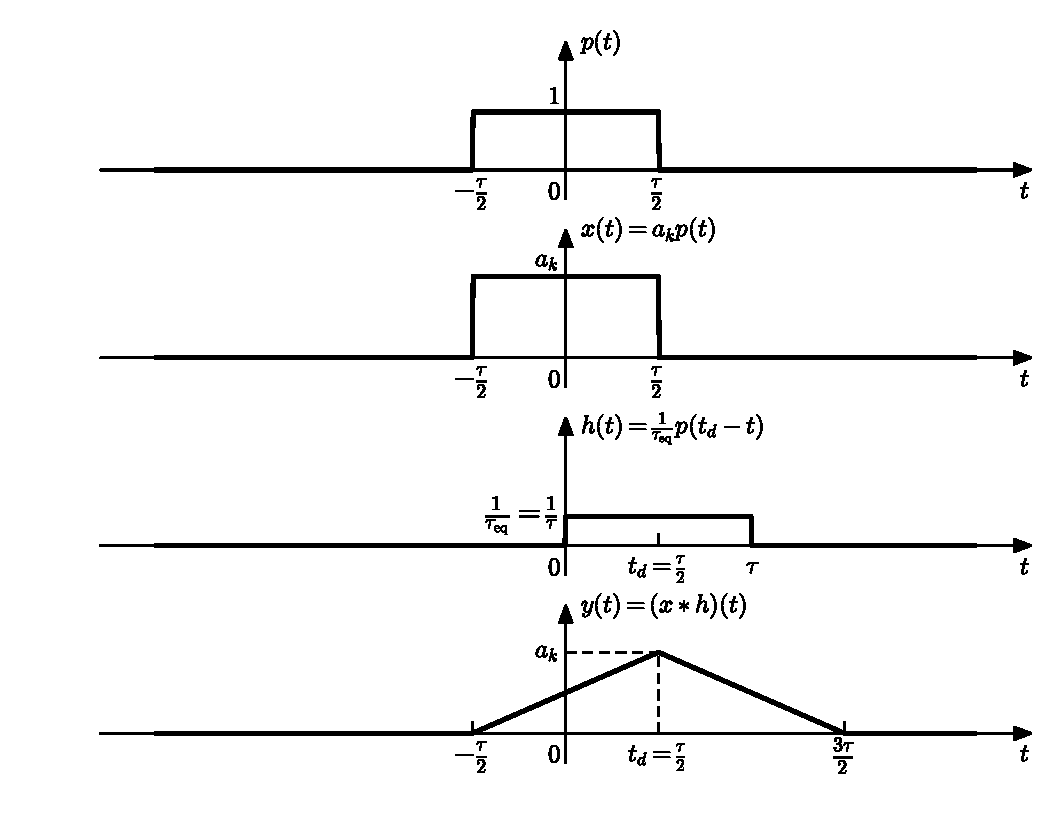
\includegraphics[width=0.9\columnwidth]{figuras/matched_filter_square_pulse_output.eps}
\caption{\label{fig:matched_filter_square_pulse_output} Respuesta del filtro acoplado a la entrada  \(x(t)=a_kp(t)\) cuando el pulso conformador \(p(t)\) es rectangular. La figura muestra respectivamente las gráficas del pulso conformador \(p(t)\), la entrada \(x(t)\), la respuesta al impulso \(h(t)\) del filtro acoplado y la salida \(y(t)\). La entrada \(x(t)\) es el pulso conformador escalado por la constante \(a_k\). La respuesta al impulso del filtro acoplado es el puso conformador invertido y desplazado \(t_d\) en el tiempo. En este ejemplo, la inversión temporal no tiene efecto debido a que el pulso conformador es una función par, es decir, se cumple que \(p(t)=p(-t)\). Notar que el desplazamiento temporal \(t_d=\tau/2\) hace que el filtro acoplado sea causal, ya que se cumple que \(h(t)=0\) si \(t<0\). La respuesta \(y(t)\) se obtiene como la convolución entre la entrada \(x(y)\) y la respuesta al impulso \(h(t)\).}
\end{center}
\end{figure}
 
\section{Potencia de señal PAM con forma de pulso arbitraria}\label{ap:pam_signal_power}
 
En este apéndice se dan indicaciones para el cálculo de la potencia de una señal PAM digital con forma de pulso conformador arbitraria. Sea una señal PAM digital \(M\)-aria con duración de símbolos de \(D\) segundos y pulso conformador \(p(t)\) limitado en el tiempo con soporte a lo sumo \(D\). El pulso \(k\)-ésimo está escalado por el número \(a_k\), que toma uno de \(M\) valores posibles para representar cada símbolo de la fuente. Como a priori no se conocen los símbolos que emitirá la fuente, \(a_k\) se modela como una variable aleatoria, y por lo tanto, la señal PAM es un proceso aleatorio.

Cómo se deduce en la sección 9.3 de \cite{lathi1990modern4th}, la función de autocorrelación de una señal PAM \(x(t)\) con las condiciones indicadas arriba es
\[
 R_x(\tau)=\frac{1}{D}\sum_{n=-\infty}^{\infty}\mathcal{R}_n\int_{-\infty}^{\infty}p(t)p(t+\tau-nD)\,dt,
\]
donde
\[
 \mathcal{R}_n=\overline{a_ka_{k+n}}.
\]
La potencia de la señal PAM es la autocorrelación evaluada en \(\tau=0\),
\[
 S_x=R_x(0)=\frac{1}{D}\sum_{n=-\infty}^{\infty}\mathcal{R}_n\int_{-\infty}^{\infty}p(t)p(t-nD)\,dt.
\]
Notando que la integral es nula para todo \(n\neq0\), se obtiene que,
\[
 S_x=\frac{1}{D}\mathcal{R}_0\int_{-\infty}^{\infty}p^2(t)\,dt,
\]
con
\[
 \mathcal{R}_0=\overline{a_k^2}.
\]
 
\section{Cálculo de la varianza de los niveles \emph{M}-arios}\label{ap:m-ary_ak_square_mean}

En este apéndice se desarrolla el cálculo de \(\overline{a_k^2}\), donde \(a_k\) es la amplitud de los niveles que toma una señal \(M\)-aria polar, y son (ecuación \ref{eq:m-ary_ak}),
\[
 a_k=\pm \frac{A}{2},\,\pm 3\frac{A}{2},\,\dots,\,\pm (M-1)\frac{A}{2},
\]
es decir,
\begin{equation}\label{eq:m-ary_ak_analitic}
 a_k=\pm(2i-1)\frac{A}{2},\qquad\textrm{con}\qquad i=1,\,\dots,\frac{M}{2}.
\end{equation}
La esperanza buscada es
\[
 \overline{a_k^2}=\sum_i\left({a_k}_i\right)^2\Pr\lbrace a_k={a_k}_i\rbrace,
\]
donde \({a_k}_i\) es el valor de amplitud que toma el nivel \(i\)-ésimo y la sumatoria es en los \(M\) niveles posibles. Asumiendo que los símbolos son equiprobables, \(\Pr\lbrace a_k={a_k}_i\rbrace=1/M\), y por lo tanto
\[
 \overline{a_k^2}=\frac{1}{M}\sum_i\left({a_k}_i\right)^2.
\]
Sustituyendo \({a_k}_i\) por el valor del nivel usando la ecuación \ref{eq:m-ary_ak_analitic}, se tiene que
\[
 \overline{a_k^2}=\frac{2}{M}\sum_{i=1}^{M/2}\left[(2i-1)\frac{A}{2}\right]^2,
\]
donde el factor de 2 proviene de que el nivel positivo y el correspondiente negativo toman el mismo valor cuando se elevan al cuadrado. Operando, se llega a que
\begin{equation}\label{eq:m-ary_ak_square_mean}
 \overline{a_k^2}=\frac{A^2}{2M}\sum_{i=1}^{M/2}(2i-1)^2.
\end{equation}
Expandiendo la sumatoria, se tiene que
\begin{align*}
 \sum_{i=1}^{M/2}(2i-1)^2&=\sum_{i=1}^{M/2}\left(4i^2-4i+1\right)\\
   &=4\sum_{i=1}^{M/2}i^2-4\sum_{i=1}^{M/2}i+\sum_{i=1}^{M/2}1.
\end{align*}
Cada sumando de la última ecuación puede calcularse empleando las identidades siguientes\footnote{\url{https://en.wikipedia.org/wiki/List_of_mathematical_series}},
\[
 \sum _{k=1}^{m}k={\frac {m(m+1)}{2}}=\frac{m^2}{2}+\frac{m}{2},\quad 
 \sum _{k=1}^{m}k^{2}={\frac {m(m+1)(2m+1)}{6}}={\frac {m^{3}}{3}}+{\frac {m^{2}}{2}}+{\frac {m}{6}},
\]
resultando cada uno en
\begin{itemize}
 \item \(\displaystyle 4\sum_{i=1}^{M/2}i^2=4\left(\frac{M^3}{8\times3}+\frac{M^2}{2\times4}+\frac{M}{2\times6}\right)=\frac{M^3}{6}+\frac{M^2}{2}+\frac{M}{3}\)
 \item \(\displaystyle -4\sum_{i=1}^{M/2}i=-4\left(\frac{M^2}{4\times2}+\frac{M}{2\times2}\right)=-\frac{M^2}{2}-M\)
 \item \(\displaystyle \sum_{i=1}^{M/2}1=\frac{M}{2}\).
\end{itemize}
Por lo tanto,
\begin{align*}
 \sum_{i=1}^{M/2}(2i-1)^2&=\frac{M^3}{6}+\frac{M}{3}-M+\frac{M}{2}\\
   &=\frac{M^3-M}{6}\\
   &=\frac{M(M^2-1)}{6},
\end{align*}
y sustituyendo este resultado en la ecuación \ref{eq:m-ary_ak_square_mean}, se obtiene que
\[
 \overline{a_k^2}=A^2\frac{(M^2-1)}{12}.
\]
 
\bibliographystyle{ieeetr}
\bibliography{matched_filter}

\end{document}
